% !TeX root = ../note.tex
\section{Используемые инструменты и технологии}\label{sec:tools}

Выбор технологий является важным предварительным этапом разработки сложных информационных систем. Платформа и язык программирования, на котором будет реализована система, заслуживает большого внимания, так как исследования показали, что выбор языка программирования влияет на производительность труда программистов и качество создаваемого ими кода~\cite{code_complete}. % page 59

Ниже перечислены некоторые факторы, повлиявшие на выбор технологий:
\begin{enumerate}
    \item Разрабатываемое ПО должно работать на дистрибутиве GNU/Linux — серверной Ubuntu 18.10;
    \item ПО требовательно к скорости работы работы технологий. По этой причине, такие языки как Python или Java не могут быть использованы;
    \item Используемый язык должен предоставлять наборы библиотек, реализующие непрофильные вещи для проекта, такие как логирование, подключение к базам данных и т.п.;
    \item Код проекта может дорабатываться другими разработчиками.
\end{enumerate}

\subsection{Golang}

Исходя из вышеперечисленных факторов можно рассмотреть лишь некоторые популярные быстрые (часто системные) языки программирования, у которых обширная база библиотек, готовых для использования, а также поддерживается платформа GNU/Linux. Таким образом круг выбора сужается до следующих языков:
\begin{itemize}
    \item C++;
    \item Rust;
    \item Scala.
    \item Golang;
\end{itemize}

Язык программирования С++ — компилируемый, статически типизированный язык программирования общего назначения. Поддерживает такие парадигмы программирования, как процедурное программирование, объектно-ориентированное программирование, обобщённое программирование. Язык имеет богатую стандартную библиотеку, которая включает в себя распространённые контейнеры и алгоритмы, ввод-вывод, регулярные выражения, поддержку многопоточности и другие возможности. C++ сочетает свойства как высокоуровневых, так и низкоуровневых языков. В сравнении с его предшественником — языком C, — наибольшее внимание уделено поддержке объектно-ориентированного и обобщённого программирования.

C++ широко используется для разработки программного обеспечения, являясь одним из самых популярных языков программирования. Область его применения включает создание операционных систем, разнообразных прикладных программ, драйверов устройств, приложений для встраиваемых систем, высокопроизводительных серверов, а также игр.

У языка C++ существует ряд проблем, вызванных историческим желанием сохранения совместимости с языком C. Синтаксис языка может вызывать проблемы в силу своей сложности, а разработчики всё реже выбирают C++ своим основным языком программирования. Поэтому C++ будет сложно поддерживать другим разработчикам. Также, несмотря на то, что у языка есть обширные библиотеки, не существует единого стандарта для их установки, поэтому у проекта с множеством зависимостей могут быть проблемы со сборкой, линковкой и несовместимостью различных библиотек.

Рассмотрим следующий вариант — язык Rust. Rust — современный мультипарадигмальный компилируемый язык программирования общего назначения. Разработка языка ведётся сообществом Mozilla Research и финансируется из фонда Mozilla Foundation. Сочетает парадигмы функционального и процедурного программирования с объектной системой, основанной на типажах. Управление памятью осуществляется через механизм ''владения`` с использованием аффинных типов, что позволяет обходиться без системы сборки мусора во время исполнения программы. Объектно-ориентированное программирование поддерживается при помощи отличных от многих языков абстракций.

Ключевые отличия языка: безопасность, скорость и параллелизм. Rust пригоден для системного программирования, в частности, используется для разработки ядер операционных систем. Rust сопоставим по скорости и возможностям с C++/Си, однако гарантирует безопасную работу с памятью, что является встроенным свойством архитектуры языка. Производительность программ на Rust обеспечивается за счёт использования ''абстракций с нулевой стоимостью``.

Rust достаточно молодой язык. Он обладает своей системой сборки и менеджером пакетов, но к сожалению на данный момент экосистема языка ещё слабо развита. Rust пока сложен в поддержке в силу своей нераспространённости, а также из-за использования нетривиальной объектной системы.

Следующий вариант — Scala. Scala — мультипарадигмальный язык программирования, спроектированный кратким и типобезопасным для простого и быстрого создания компонентного программного обеспечения, сочетающий возможности функционального и объектно-ориентированного программирования. Scala является достаточно производительным языком, но в силу необычности своего проектирования (сочетает как функциональную, так и объектную модели), используется он гораздо реже C++ и Golang, и разработчиков на Scala довольно мало. Разработчик данного дипломного проекта также не владеет этим языком. Остался последний вариант — язык Golang.

Go (часто также Golang) — компилируемый многопоточный язык программирования, разработанный внутри компании Google. Разработка Go началась в сентябре 2007 года, его непосредственным проектированием занимались Роберт Гризмер, Роб Пайк и Кен Томпсон. Официально язык был представлен в ноябре 2009 года. На данный момент поддержка официального компилятора, разрабатываемого создателями языка, осуществляется для операционных систем FreeBSD, OpenBSD, Linux, macOS, Windows и других. Также Go поддерживается набором компиляторов gcc, существует несколько независимых реализаций. Ведётся разработка второй версии языка~\cite{golang}.

Язык Go разрабатывался как язык программирования для создания высокоэффективных программ, работающих на современных распределённых системах и многоядерных процессорах. Он может рассматриваться как попытка создать замену языкам Си и C++ с учётом изменившихся компьютерных технологий и накопленного опыта разработки крупных систем. По словам Роба Пайка, ``Go был разработан для решения реальных проблем, возникающих при разработке программного обеспечения в Google''.

Go создавался в расчёте на то, что программы на нём будут транслироваться в объектный код и исполняться непосредственно, не требуя виртуальной машины, поэтому одним из критериев выбора архитектурных решений была возможность обеспечить быструю компиляцию в эффективный объектный код и отсутствие чрезмерных требований к динамической поддержке.

Go не содержит целого ряда популярных синтаксических средств, доступных в других современных языках прикладного программирования. Во многих случаях это вызвано сознательным решением разработчиков. В частности:

\begin{itemize}
    \item Структурная запись обработчиков исключений сочтена провоцирующей на пропуск ошибок или неадекватную их обработку. К тому же поддержка исключений серьёзно усложняется в приложениях с параллельно работающими частями. Вместо неё предлагается проверка кодов возврата с использованием многозначных функций и специального интерфейса error, а также применение отложенных (deferred) функций для перехвата исключительных ситуаций.
    \item Наследование реализации, как считают авторы, приводит к созданию кода с неявными зависимостями, избыточно сложного в поддержке. Аналогичные возможности, но без свойственных наследованию нежелательных эффектов, обеспечиваются поддержкой вложения типов и свободно определяемыми интерфейсами.
    \item Обобщённое программирование. Авторы воздержались от его включения в первую версию языка, поскольку, по их словам, предоставляемые им возможности не окупают требуемого усложнения компилятора и runtime-библиотек, а уже имеющиеся в языке средства (пустые интерфейсы, «утиная типизация» и рефлексия) позволяют создавать обобщённый код без специальных синтаксических механизмов. Тем не менее, обсуждается вопрос о включении таких средств в проектируемую вторую версию языка.
    \item Использование утверждений (assertion) было сочтено ненужным.
    \item Переопределение методов и функций было исключено из соображений надёжности и эффективности компиляции: требование различного именования всех методов на одном уровне видимости устраняет необходимость сопоставлять списки параметров при компиляции вызовов функций и методов и исключает ошибочный вызов другого одноимённого метода; при этом сама возможность переопределения есть не более чем синтаксический сахар.
    \item Ряд операций над массивами и срезами (например, вставка элемента в середину) не включен в язык, поскольку они достаточно затратны. Возможность их выполнения одной простой командой провоцировала бы программиста на создание неэффективного кода, отсутствие таких команд в языке, напротив, является стимулом для рассмотрения альтернативных решений.
    \item Поддержка отрицательных индексов, доступная в ряде популярных языков, может стать причиной труднообнаруживаемых ошибок: появление отрицательного индекса из-за ошибки в коде вместо того, чтобы привести к фатальному сбою, вызовет внешне корректное обращение не к тем элементам массива, что проявится только в неверных результатах и может быть обнаружено далеко не сразу.
    \item Принцип «любое выражение возвращает значение» провоцирует программиста на создание сложных, трудно воспринимаемых и чреватых неочевидными ошибками выражений (вроде копирования строки на Си командой из трёх слов: while (*ptr1++ = *ptr2++);). При этом современные технологии оптимизации обеспечат одинаковый объектный код и для экстремально сокращённого выражения, и для аналогичного ему фрагмента, написанного безо всяких ухищрений.
\end{itemize}

Далее рассмотрим некоторые особенности и полезные пакеты языка Golang.

% \subsubsection{} Пакеты
\textbf{Пакеты}

Любая программа на Go включает один или несколько пакетов. Пакет, к которому относится файл исходного кода, задаётся описанием package в начале файла. Имена пакетов имеют те же ограничения, что и идентификаторы, но могут содержать буквы только нижнего регистра. Система пакетов go-среды имеет древовидную структуру, аналогичную дереву каталогов. Любые глобальные объекты (переменные, типы, интерфейсы, функции, методы, элементы структур и интерфейсов) доступны без ограничений в пакете, в котором они объявлены. Глобальные объекты, имена которых начинаются на заглавную букву, являются экспортируемыми.

% \subsubsection{} Механизм отложенного вызова defer
\textbf{Механизм отложенного вызова defer}

Отложенный вызов заменяет сразу несколько синтаксических средств, в частности, обработчики исключений и блоки с гарантированным завершением. Вызов функции, которому предшествует ключевое слово defer, параметризуется в той точке программы, где размещён, а выполняется непосредственно перед выходом программы из области видимости, где он был объявлен, независимо от того, как и по какой причине происходит этот выход. Если в одной функции содержится несколько объявлений defer, соответствующие вызовы выполняются по завершении функции последовательно, в обратном порядке.

% \subsubsection{} Обработка ошибок и исключительных ситуаций
\textbf{Обработка ошибок и исключительных ситуаций}

Язык Go не поддерживает типичного для большинства современных языков синтаксиса структурной обработки исключений, предполагающего генерацию исключений специальной командой (обычно throw или raise) и их обработку в блоке try-catch. Вместо этого рекомендуется использовать возврат ошибки как одного из результатов функции (что достаточно удобно, так как в Go функция может возвращать более одного значения):

В последнем параметре функция возвращает объект-ошибку либо пустой указатель nil, если функция выполнилась без ошибок. В качестве типа ошибки обычно используется библиотечный интерфейс error.
Возвращённый функцией объект проверяется и ошибка, если она возникла, обрабатывается. Если ошибка в месте вызова не может быть адекватно обработана, она обычно возвращается в качестве результата текущей функции, либо на её основе создаётся новая ошибка, которая и возвращается.

% \subsubsection{} Многопоточность
\textbf{Многопоточность}

Go дает возможность создать новый поток выполнения программы с помощью ключевого слова \lstinline{go}, которое запускает анонимную или именованную функцию в заново созданной go-процедуре (термин, используемый в Go для обозначения сопрограмм). Все go-процедуры в рамках одного процесса используют общее адресное пространство, выполняясь над ОС-потоками, но без жёсткой привязки к последним, что позволяет выполняющейся go-процедуре покидать поток с заблокированной go-процедурой (ждущей, например, отправки или приема сообщения из канала) и продолжать работу далее. Библиотека времени исполнения включает мультиплексор, обеспечивающий разделение доступного количества системных ядер между go-процедурами. Имеется возможность ограничить максимальное число физических процессорных ядер, на которых будет исполняться программа. Самостоятельная поддержка go-процедур runtime-библиотекой Go позволяет без затруднений использовать в программах огромные количества go-процедур, намного превышающие предельное число поддерживаемых системой потоков.

Для связи между go-процедурами используются каналы (встроенный тип \lstinline{chan}), через которые можно передавать любые значения. Канал создаётся встроенной функцией \lstinline{make()}, которой передаётся тип и (опционально) объём канала. По умолчанию объём канала равен нулю. Такие каналы являются небуферизованными. Можно задать любой целый положительный объём канала, тогда будет создан буферизованный канал.

% \subsubsection{} log15
\textbf{log15}

log15 — библиотека для структурированного составного логирования в Golang~\cite{log15}. Пакет log15 предоставляет простой и понятный инструментарий, использующий best-practice приёмы логирования в Go (golang), которые удобны для чтения человеком и машиной. Он создан по образцу пакетов io и net/http стандартной библиотеки Go и является альтернативой пакету журналов стандартной библиотеки.

Из особенностей библиотеки можно отметить:
\begin{itemize}
    \item простой и понятный программный интерфейс;
    \item логирование структурировано благодаря использованию пар ключ-значение;
    \item существует наследование логгеров с созданием приватного контекста у наследника;
    \item для дорогостоящих операций используется ``ленивое вычисление'';
    \item поддержка цветов терминала;
    \item встроенная поддержка записи в файлы, потоки, syslog, а также по сети.
\end{itemize}

% \subsubsection{} pflag и viper
\textbf{pflag и viper}

pflag — альтернатива стандартной библиотеке flag. Имеет совместимый интерфейс с flag. Важной особенностью, ставшей поводом для использования, является возможность добавлять POSIX/GNU флаги, которые начинаются с двух дефисов: \lstinline{--flag}.

Также важной особенностью библиотеки pflag является совместимость с другой библиотекой, использующейся для конфигурации — viper~\cite{viper}. Список полезных функций viper включает в себя:
\begin{itemize}
    \item настройка значений по умолчанию;
    \item работа с форматами JSON, YAML и другими;
    \item чтение из переменных окружения;
    \item интеграция с флагами командной строки (pflag);
\end{itemize}

\subsection{RabbitMQ}

Для разработки системы надёжного обмена данными между сервисами необходимо использовать какую-либо прослойку, умеющую работать между процессами и гарантирующую доставку данных. Для таких целей подойдёт технология ``очереди сообщений''.

Очередь сообщений — программно-инженерный компонент, используемый для межпроцессного или межпотокового взаимодействия внутри одного процесса. Для обмена сообщениями используется очередь.

Очереди сообщений предоставляют асинхронный протокол передачи данных, означая, что отправитель и получатель сообщения не обязаны взаимодействовать с очередью сообщений одновременно. Размещённые в очереди сообщения хранятся до тех пор, пока получатель не получит их.

Очереди сообщений имеют неявные или явные ограничения на размер данных, которые могут передаваться в одном сообщении, и количество сообщений, которые могут оставаться в очереди.

Многие реализации очередей сообщений функционируют внутренне: внутри операционной системы или внутри приложения. Такие очереди существуют только для целей этой системы. Другие реализации позволяют передавать сообщения между различными компьютерными системами, потенциально подключая несколько приложений и несколько операционных систем. Эти системы очередей сообщений обычно обеспечивают расширенную функциональность для обеспечения устойчивости, чтобы гарантировать, что сообщения не будут «потеряны» в случае сбоя системы.

Исторически очередь сообщений использовала собственные закрытые протоколы, которые ограничивали способность различных операционных систем или языков программирования взаимодействовать в гетерогенном множестве сред.

Появились три стандарта, которые используются в реализациях очереди сообщений с открытым исходным кодом:

\begin{itemize}
    \item Advanced Message Queuing Protocol (AMQP) — многофункциональный протокол очереди сообщений
    \item STOMP  — простой текстовый протокол сообщений
    \item MQTT — протокол облегчённой очереди сообщений, особенно для встроенных устройств
\end{itemize}

В данном дипломном проекте используется протокол AMQP и его реализация в RabbitMQ.

RabbitMQ — программный брокер сообщений на основе стандарта AMQP — тиражируемое связующее программное обеспечение, ориентированное на обработку сообщений. Создан на основе системы Open Telecom Platform, написан на языке Erlang, в качестве движка базы данных для хранения сообщений использует Mnesia.

Состоит из сервера, библиотек поддержки протоколов HTTP, XMPP и STOMP, клиентских библиотек AMQP для Java и .NET Framework и различных плагинов (таких как плагины для мониторинга и управления через HTTP или веб-интерфейс или плагин ``Shovel'' для передачи сообщений между брокерами). Имеется реализация клиентов для доступа к RabbitMQ для целого ряда языков программирования, в том числе для Perl, Python, Ruby. Поддерживается горизонтальное масштабирование для построения кластерных решений.


\subsection{Redis}

Для создания событий, которые генерируются одним сервисом и прослушиваются другим, можно использовать RabbitMQ и его очередь сообщений, но у так подхода есть два существенных недостатка:
\begin{enumerate}
    \item прослушивать такие события сможет только один участник, так как если сообщение будет вычитано из очереди, то другие не смогут его прочитать, а это недопустимо в системе с кластером похожих сервисов;
    \item неэффективная трата памяти на пересылку сообщений, так как они не несут в себе полезной информации, а в очереди придётся хранить как минимум название сообщения.
\end{enumerate}

Для решения проблем системы событий рассмотрим шаблон проектирования ``издатель-подписчик'' или pub/sub (publisher/subscriber).

Издатель-подписчик — поведенческий шаблон проектирования передачи сообщений, в котором отправители сообщений, именуемые издателями (publishers), напрямую не привязаны программным кодом отправки сообщений к подписчикам (subscribers). Вместо этого сообщения делятся на классы и не содержат сведений о своих подписчиках, если таковые есть. Аналогичным образом подписчики имеют дело с одним или несколькими классами сообщений, абстрагируясь от конкретных издателей~\cite{patterns}.

Шаблон издатель-подписчик представляет собой расширение шаблона наблюдатель, в который добавлено описание канала событий (event channel), специально предназначенного для оповещения о событиях. Шаблон издатель-подписчик наряду с близкой ему концепцией очереди сообщений содержится в арсенале средств событийно-ориентированного промежуточного слоя ПО большой системы. Большинство систем передачи сообщений поддерживают в своем API как и модель издатель-подписчик, так и очередь сообщений.

Реализация шаблона pub/sub в Redis подходит для использования в данном дипломном проекте.

Redis (remote dictionary server) — резидентная система управления базами данных класса NoSQL с открытым исходным кодом, работающая со структурами данных типа ``ключ — значение''. Используется как для баз данных, так и для реализации кэшей, брокеров сообщений~\cite{redis}.

Ориентирована на достижение максимальной производительности на атомарных операциях (приблизительно 100 тыс. SET- и GET-запросов в секунду на Linux-сервере начального уровня). Написана на Си, интерфейсы доступа созданы для большинства основных языков программирования.

Реализация pub/sub в Redis обладает необходимыми функциями, высокой скоростью работы и может использоваться как для межпроцессной коммуникации, так и для работы через сеть.

\subsection{MongoDB}

Данные в проекте обладают малой связностью, поэтому использование привычных реляционных баз данных нецелесообразно. Для хранения данных об ордерах и балансах лучше использовать базу данных, ориентированную на высокую скорость записи и обновления данных. Примером такой базы данных является MongoDB.

MongoDB — документоориентированная система управления базами данных с открытым исходным кодом, не требующая описания схемы таблиц. Классифицирована как NoSQL, использует JSON-подобные документы и схему базы данных. Написана на языке C++~\cite{mongo}.

Система поддерживает ad-hoc-запросы: они могут возвращать конкретные поля документов и пользовательские JavaScript-функции. Поддерживается поиск по регулярным выражениям. Также можно настроить запрос на возвращение случайного набора результатов.

Система масштабируется горизонтально, используя технику сегментирования (sharding) объектов баз данных — распределение их частей по различным узлам кластера. Администратор выбирает ключ сегментирования, который определяет, по какому критерию данные будут разнесены по узлам (в зависимости от значений хэша ключа сегментирования). Благодаря тому, что каждый узел кластера может принимать запросы, обеспечивается балансировка нагрузки.

MongoDB целесообразно использовать также по причине её популярности в веб-разработке. Так как проект ориентирован на дальнейшее расширение через front-end, то MongoDB будет удобна для веб-разработчиков.

\subsection{Clickhouse}

Следующим пунктом необходимо выбрать базу данных для хранения сделок. Данные, которые должны храниться в данной БД, обладают некоторыми отличиями от того, что обычно хранят в БД:
\begin{itemize}
    \item сделки постоянно добавляются с растущим временем создания;
    \item сделки не удаляются и не обновляются.
\end{itemize}

Для хранения данных с такими характеристиками можно рассматривать два типа баз: колоночные и временные. Выбор был сделан в пользу колоночной СУБД, так как сделки хранятся не по временным срезам, а по идентификатору. В качестве СУБД выбрана ClickHouse.

ClickHouse — это колоночная аналитическая СУБД с открытым кодом, позволяющая выполнять аналитические запросы в режиме реального времени на структурированных больших данных, разрабатываемая компанией Яндекс~\cite{clickhouse}.

ClickHouse использует собственный диалект SQL близкий к стандартному, но содержащий различные расширения: массивы и вложенные структуры данных, функции высшего порядка, вероятностные структуры, функции для работы с URI, возможность для работы с внешними key-value хранилищами («словарями»), специализированные агрегатные функции, функциональности для семплирования, приблизительных вычислений, возможность создания хранимых представлений с агрегацией, наполнения таблицы из потока сообщений Apache Kafka и т. д.

Однако при этом имеются и ограничения — отсутствие транзакций, отсутствие точечных UPDATE/DELETE (пакетный UPDATE/DELETE был введен в июне 2018 года), ограниченная поддержка синтаксиса JOIN, строгие типы с необходимостью явного приведения, для некоторых операций промежуточные данные должны помещаться в оперативную память, отсутствие оконных функций, отсутствие полноценного оптимизатора запросов, точечного чтения, присутствие ограничений в реализации некоторых функций, связанных со спецификой использования ClickHouse в Яндексе, и т. д.

Система оптимизирована для хранения данных на жестких дисках (используются преимущества линейного чтения, сжатия данных). Для обеспечения отказоустойчивости и масштабируемости ClickHouse может быть развернут на кластере (для координации процесса репликации используется Apache ZooKeeper). Для работы с базой данных существует консольный клиент, веб-клиент, HTTP интерфейс, ODBC и JDBC-драйверы, а также готовые библиотеки для интеграции со многими популярными языками программирования и библиотеками.

\subsection{Protobuf}

Для передачи данных необходим единый формат сериализации данных. В данный одним из самых популярных и эффективных форматов является protobuf.

Protocol Buffers — протокол сериализации (передачи) структурированных данных, предложенный Google как эффективная бинарная альтернатива текстовому формату XML. Разработчики сообщают, что Protocol Buffers проще, компактнее и быстрее, чем XML, поскольку осуществляется передача бинарных данных, оптимизированных под минимальный размер сообщения~\cite{protobuf}.

По замыслу разработчиков, сначала должна быть описана структура данных, которая затем компилируется в классы. Вместе с классами идёт код их сериализации в компактном формате представления. Чтение и запись данных доступна в высокоуровневых языках программирования — таких как Java, C++ или Python.

Protocol Buffers не предназначен для чтения пользователем и представляет собой двоичный формат. Для десериализации данных необходим отдельный .proto-файл, в котором определяется формат сообщения.

% TODO: proto style
\lstinputlisting[caption=Пример proto-файла]{appendix/protobuf.proto}

\subsection{gRPC}

Для работы с пользователями в сервисе авторизации удобно использовать технологию RPC — удалённый вызов процедур. В данном проекте будет использоваться реализация от компании Google — gRPC фреймворк.

gRPC — это высокопроизводительный фреймворк для вызова удаленных процедур (RPC), который работает поверх протокола HTTP/2~\cite{grpc}.

gRPC простой в использовании, отлично подходит для создания распределенных систем (микросервисов) и API. Имеет встроенную поддержку для балансировки нагрузки, трассировки, аутентификации и проверки жизнеспособности сервисов. Есть возможность создавать клиентские библиотеки для работы с back-end на 10 языках. Высокая производительность достигается за счет использования протокола HTTP/2 и Protocol Buffers.

Одной из сильнейших сторон фреймворка является наличие разных типов связи:
\begin{itemize}
    \item Унарный (Unary RPC). Синхронный запрос клиента, который блокируются пока не будет получен ответ от сервера.
    \item Серверный стрим (Server streaming RPC), при подключении клиента сервер открывает стрим и начинает отправлять сообщения.
    \item Клиентский стрим (Client streaming RPC). То же самое, что и серверный, только клиент начинает стримить сообщения на сервер.
    \item Двунаправленный стрим (Bidirectional streaming). Клиент инициализирует соединение, создаются два стрима. Сервер может отправить изначальные данные при подключении или отвечать на каждый запрос клиента по типу “пинг-понга”.
\end{itemize}

\subsection{JWT}

Авторизация пользователей будет происходить с использованием стандарта JWT~\cite{jwt}.

JSON Web Token (JWT) — это открытый стандарт (RFC 7519) для создания токенов доступа, основанный на формате JSON. Как правило, используется для передачи данных для аутентификации в клиент-серверных приложениях. Токены создаются сервером, подписываются секретным ключом и передаются клиенту, который в дальнейшем использует данный токен для подтверждения своей личности.

Токен JWT состоит из трех частей: заголовка (header), полезной нагрузки (payload) и подписи или данных шифрования. Первые два элемента — это JSON объекты определенной структуры. Третий элемент вычисляется на основании первых и зависит от выбранного алгоритма (в случае использования не подписанного JWT может быть опущен). Токены могут быть перекодированы в компактное представление (JWS/JWE Compact Serialization): к заголовку и полезной нагрузке применяется алгоритм кодирования Base64-URL, после чего добавляется подпись и все три элемента разделяются точками (``.'').

К примеру, для заголовка и полезной нагрузки, которые выглядят следующим образом:

\begin{lstlisting}[language=javascript]
{
  "alg": "HS512",
  "typ": "JWT"
}
{
  "sub": "12345",
  "name": "John Gold",
  "admin": true
}
\end{lstlisting}

Получим следующее компактное представление (переводы строки добавлены для наглядности):

\begin{lstlisting}
eyJhbGciOiJIUzUxMiIsInR5cCI6IkpXVCJ9.
eyJzdWIiOiIxMjM0NSIsIm5hbWUiOiJKb2hu
IEdvbGQiLCJhZG1pbiI6dHJ1ZX0K.
LIHjWCBORSWMEibq-tnT8ue\_deUqZx1K0XxCOXZRrBI
\end{lstlisting}

\subsection{Docker}

В современном мире при разработке ПО, состоящего из множества отдельных сервисов, принято создавать образы в docker и docker-compose для быстрого развёртывания всех сервисов и налаживания связей между ними.

Docker — программное обеспечение для автоматизации развёртывания и управления приложениями в средах с поддержкой контейнеризации. Позволяет ``упаковать'' приложение со всем его окружением и зависимостями в контейнер, который может быть перенесён на любую Linux-систему с поддержкой cgroups в ядре, а также предоставляет среду по управлению контейнерами. Изначально использовал возможности LXC, с 2015 года применял собственную библиотеку, абстрагирующую виртуализационные возможности ядра Linux — libcontainer. Схема архитектуры представлена на рис.~\ref{fig:docker}.

\begin{figure}[ht]
    \centering
    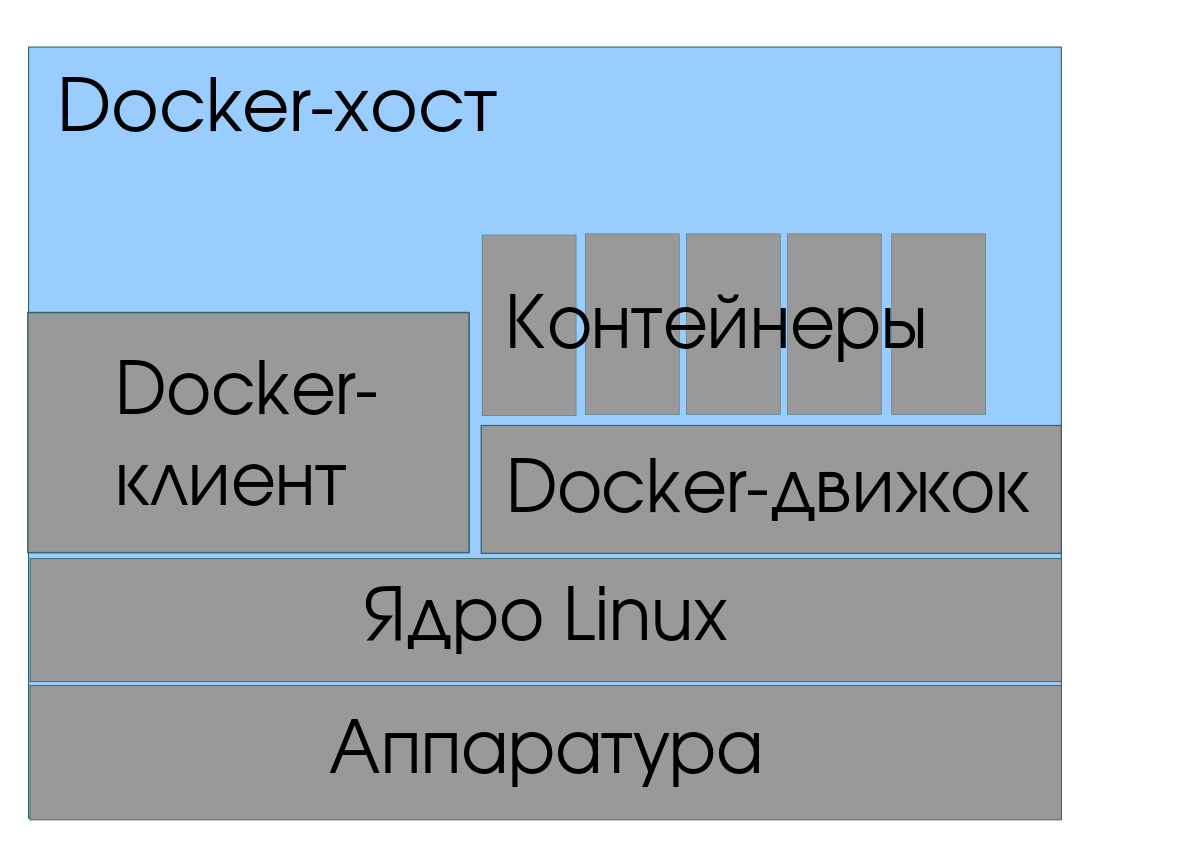
\includegraphics[scale=0.25]{docker.png}
    \caption{Docker на физическом linux-сервере}\label{fig:docker}
\end{figure}

В состав программных средств входит демон — сервер контейнеров (запускается командой docker -d), клиентские средства, позволяющие из интерфейса командной строки управлять образами и контейнерами, а также API, позволяющий в стиле REST управлять контейнерами программно.

Набор клиентских средств позволяет запускать процессы в новых контейнерах (docker run), останавливать и запускать контейнеры (docker stop и docker start), приостанавливать и возобновлять процессы в контейнерах (docker pause и docker unpause). Серия команд позволяет осуществлять мониторинг запущенных процессов (docker ps по аналогии с ps в Unix-системах, docker top по аналогии с top и другие). Новые образы возможно создавать из специального сценарного файла (docker build, файл сценария носит название Dockerfile), возможно записать все изменения, сделанные в контейнере, в новый образ (docker commit). Все команды могут работать как с docker-демоном локальной системы, так и с любым сервером Docker, доступным по сети. Кроме того, в интерфейсе командной строки встроены возможности по взаимодействию с публичным репозиторием Docker Hub, в котором размещены предварительно собранные образы контейнеров, например, команда docker search позволяет осуществить поиск образов среди размещённых в нём, образы можно скачивать в локальную систему (docker pull), возможно также отправить локально собранные образы в Docker Hub (docker push).


Также в Docker присутствует пакетный менеджер docker-compose, который позволяет описывать и запускать многоконтейнерные приложения. Конфигурационные файлы для docker-compose описываются на языке YAML.
